\documentclass[12pt,pdftex]{article}
\usepackage[utf8]{inputenc}
\usepackage[T1,T2A]{fontenc}
\usepackage[english,russian]{babel}
\usepackage[table,xcdraw]{xcolor}
\usepackage[left=2.5cm,right=2.5cm, top=2cm,bottom=2cm]{geometry}

\RequirePackage{
,amsmath
,amssymb
,array
,comment
,csquotes
,dsfont
,enumerate
,fancyhdr
,graphicx
,icomma
,indentfirst
,mathtext
,multicol
,pdfpages
,pgfplots
,pgfplotstable
,refstyle
,textcomp
,tikz
,verbatim
,wrapfig
}

\DeclareUnicodeCharacter{2014}{\dash}
%делаю символ чтд

\pagestyle{empty} 
\setcounter{page}{0}
%нумерация страниц

\graphicspath{{pics/}} 
%дириктория с картинками 

\pgfplotsset{compat=1.16} 
%штука для графиков

\newcolumntype{C}[1]{>{\centering\let\newline\\\arraybackslash\hspace{0pt}}m{#1}}
%для фиксированых колонок в таблицах

\begin{comment}
\renewcommand\thesection{\arabic{section}.\arabic{subsection}}
\renewcommand\thesubsection{\arabic{section}.\arabic{subsection}}
\setcounter{section}{-1}
\end{comment}
%секции подсекции и вот это всё говно

\begin{document}

\section*{2}
Составим двудольный граф таким образом, что левая доля это столбы а правая это строки, ребро между вершинами есть если на пересечении этого столбца и этой строки стоит положительное число. По теореме Кёнига, мы знаем, что наибольшее паросочетание (то что нас просят найти) равно наименьшему вершинному покрытию. Докажем что последнее равно $n$. Понятно что за $n$ мы справимся (просто выделим все вершины в одной доле), докажем что за меньшее количество нельзя. Пусть мы составили вершинное покрытие из $k<n$ вершин. Тогда сумма чисел на ребрах покрытых этими вершинами $\leq k = k \cdot 1$, т. к. если ребро покрыто два раза, то оно учитывается только один раз, а сумма чисел под ребрами для каждой вершины равна $1$. Но с другой стороны сумма чисел во всей таблице равна $n > k$, противоречие. Следовательно наименьшее вершинное покрытие равно $n$ равно наибольшему паросочетанию ч.т.д.

\section*{4 Прямая Гаусса}
\begin{wrapfigure}{r}{0.4\linewidth}
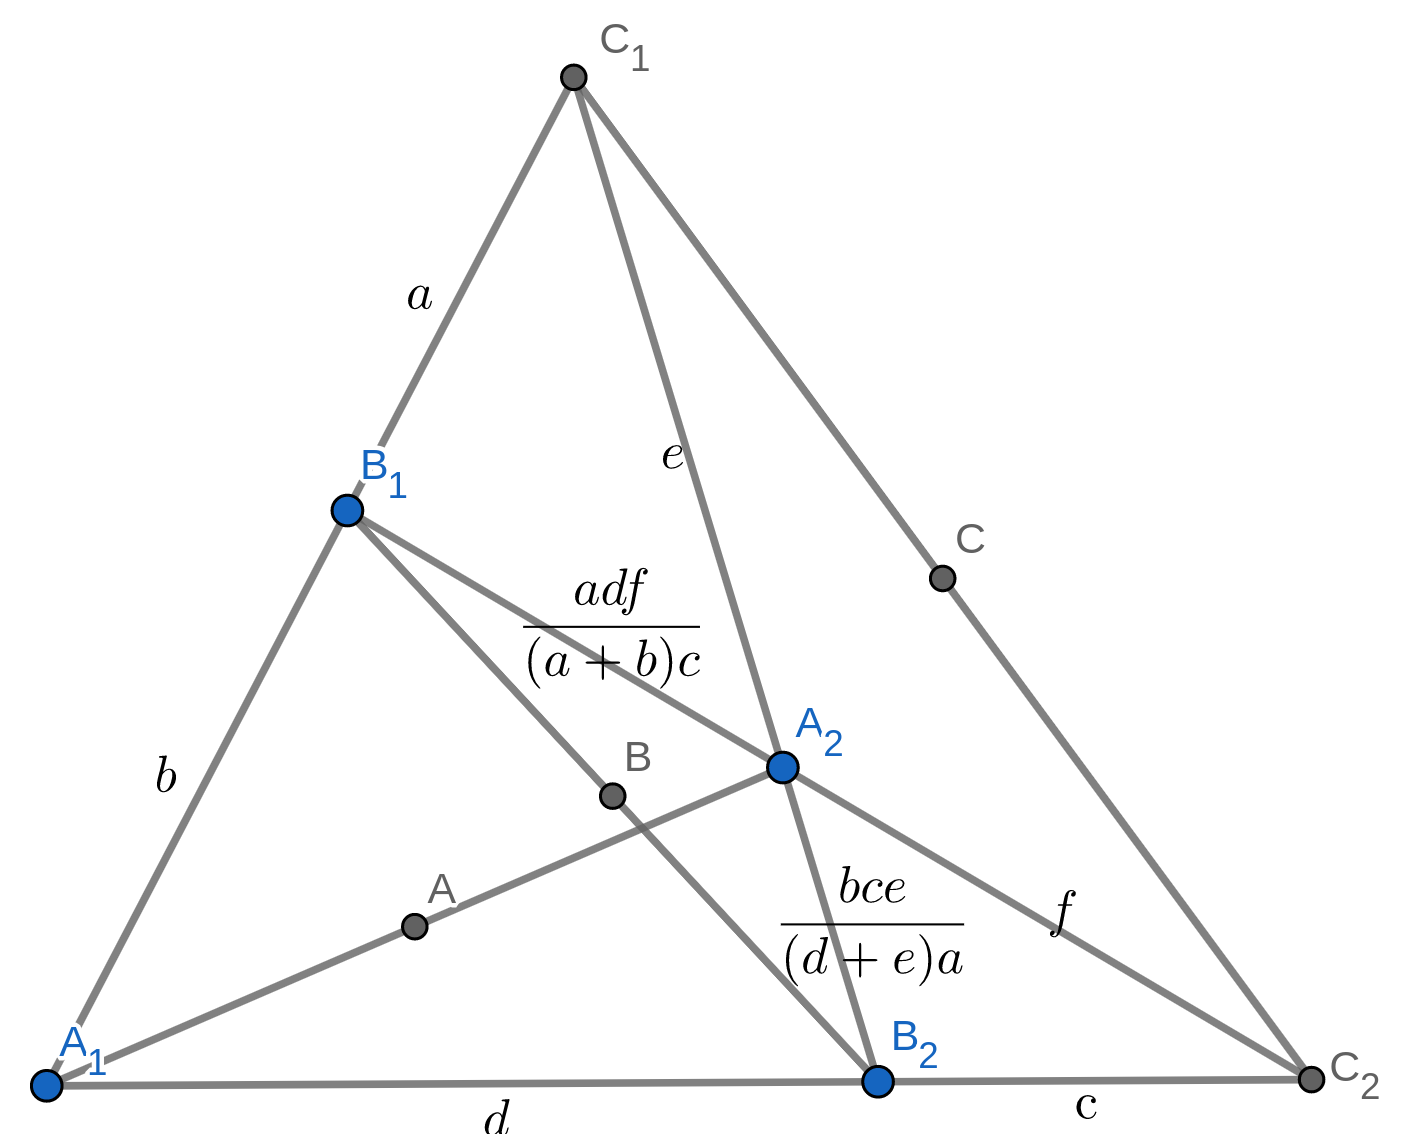
\includegraphics[width=\linewidth]{tasks/Гаусс жив.png}
\end{wrapfigure}

Пускай отрезки имеют длины такие же какие указаны на рисунке (длины отрезков $B_1A_2$ и $B_2A_2$ вычислены из других с помощью теоремы Менелая). Тогда поставим массу $-\frac{2bc}{a(c+d)} =(-\frac{bc}{ad}) +  \frac{bc(c-d)}{ad(c+d)}$ в $C_1$,
$-\frac{2bc}{a(c+d)} = -\frac{2bc+ac+ad}{a(c+d)} + 1$ в $C_2$,
$\frac{2c(a+b)}{ad} = \frac{c(a+b)}{ad} + \frac{c(a+b)}{ad}$ в  $B_1$
и $\frac{2c(a+b)}{ad} = \frac{ad+2bc+ac}{ad} + \frac{c-d}{d}$ в $B_2$. Тогда, т. к. в вершинах $C_1$ и  $C_2$ находятся одинаковые массы, заменим их на их центр масс в точке $C$. Аналогично заменим $B_1$ и  $B_2$ на $B$. Таким образом центр масс системы из этих четырех точек лежит на прямой $BC$, найдем его. 

Для этого найдем центр масс части точки $C_1$ с массой $(-\frac{bc}{ad})$ и части точки $B_1$ с массой $\frac{c(a+b)}{ad}$. Это точка $A_1$, т. к. $A_1B_1 \cdot \frac{c(a+b)}{ad} + A_1C_1 \cdot (-\frac{bc}{ad})= \frac{abc+b^2c}{ad} -\frac{abc + b^2c}{ad} = 0$. Также для части точки $C_2$ с массой $(-\frac{2bc+ac+ad}{a(c+d)})$ и части точки $B_2$ с массой $\frac{ad+2bc+ac}{ad}$ центр масс также $A_1$, т. к. $A_1B_2 \cdot \frac{ad+2bc+ac}{ad} + A_1C_2 \cdot (-\frac{2bc+ac+ad}{a(c+d)})= \frac{ad+2bc+ac}{a} -\frac{2bc+ac+ad}{a} = 0$. Таким образом в точке $A_1$ скопилась сумма этих масс, а именно масса $-\frac{bc}{ad}-\frac{2bc+ac+ad}{a(c+d)}+\frac{c(a+b)}{ad}+\frac{ad+2bc+ac}{ad}=\frac{2c(a+b)}{ad}+1-\frac{2bc+ac+ad}{a(c+d)}=\frac{2c(ac+ad+bc)}{ad(c+d)}$. Для оставшихся частей масс в точках также найдем их центр. Для части точки $C_1$ с массой $\frac{bc(c-d)}{ad(c+d)}$ и части точки $B_2$ с массой $\frac{c-d}{d}$ это точка $A_2$, т. к. $C_1A_2 \cdot \frac{bc(c-d)}{ad(c+d)} = \frac{bce(c-d)}{ad(c+d)} = A_2B_2 \cdot \frac{c-d}{d}$. Осталось найти центр масс части точки $B_1$ с массой $\frac{c(a+b)}{ad}$ и части точки $C_2$ с массой $1$, это точка $A_2$, т. к. $B_1A_2 \cdot \frac{c(a+b)}{ad} = f = A_2C_2 \cdot 1$. Таким образом в точке $A_1$ скопилась сумма этих масс, а именно масса $\frac{bc(c-d)}{ad(c+d)} + \frac{c-d}{d} + \frac{c(a+b)}{ad} + 1 = \frac{c}{d}(\frac{b(c-d)}{a(c+d)} + 1 + \frac{(a+b)}{a}) = (\frac{c}{d})\frac{bc-bd+ac+ad+ac+bc+ad+bd}{a(c+d)} = \frac{2c(ac+ad+bc)}{ad(c+d)}$. 

\begin{wrapfigure}{r}{0.05\linewidth}

\includegraphics[width=\linewidth]{tasks/SXKj17wSmm.png}
\end{wrapfigure}

Мы свели нашу систему точек к двум точкам $A_1$ и $A_2$ с равными массами, значит центр масс системы находится в середине отрезка $A_1A_2$ в точке $A$. 
Ранее мы доказали, что центр масс лежит на прямой $BC$, тогда $A$ лежит на прямой $BC$ ч. т. д.

%\frac{bc^2-bcd+ac^2-ad^2 + ac^2 +acd+bc^2+bcd + acd + ad^2}{ad(c+d)} = \frac{ac^2 + ac^2 +acd+ acd}{ad(c+d)}=\frac{2c(c +d)}{ad(c+d)}=\frac{2c}{ad}$



\section*{5 Йенсен}
Пусть мы знаем, что для любых двух точек $x_1$ и $x_2$ и выпуклой вниз функции $f(x)$, а также любых двух чисел $q_1$ и $q_2 \geq 0$, таких что $q_1+q_2=1$ выполнено $q_1f(x_1)+q_2f(x_2) \geq f(q_1x_1+ q_2x_2)$ (определение выпуклости). Предположим, что для любых $x_1, x_2, ..., x_n$, выпуклой вверх функции $f(x)$ и любых $q_1, q_2, ..., q_n \geq 0$, т. ч. $\sum_{i=1}^n q_i = 1$ выполнено $\sum_{i=1}^n q_if(x_i) \geq f(\sum_{i=1}^n q_ix_i)$. Докажем, что и для любых $x_1, x_2, ..., x_{n+1}$, этой же функции $f(x)$ и любых $q_1, q_2, ..., q_{n+1} \geq 0$, т. ч. $\sum_{i=1}^{n+1} q_i = 1$ выполнено $\sum_{i=1}^{n+1} q_if(x_i) \geq f(\sum_{i=1}^{n+1} q_ix_i)$. Из предположения следует $(q_1+q_2)f(\frac{q_1x_1 + q_2x_2}{q_1+q_2}) + ... + q_{n+1}f(x_{n+1}) \geq f((q_1+q_2)\frac{q_1x_1 + q_2x_2}{q_1+q_2} + ...  + q_{n+1}x_{n+1})$. Сравним левую часть этого неравенства с $\sum_{i=1}^{n+1} q_if(x_i)$, удалив все повторяющиеся члены получим, что должно выполняться: $q_1f(x_1)+q_2f(x_2) \geq (q_1+q_2)f(\frac{q_1x_1 + q_2x_2}{q_1+q_2})$ Поделим на $q_1+q_2$, получим $\frac{q_1}{q_1+q_2}f(x_1)+\frac{q_2}{q_1+q_2}f(x_2) \geq f(x_1\frac{q_1}{q_1+q_2} + x_2\frac{q_2}{q_1+q_2})$, что правда по определению выпуклости, т. к. $\frac{q_1}{q_1+q_2} + \frac{q_2}{q_1+q_2} = 1$.


\end{document}
